\section{Clustering-based naming}
\label{sec:clustering}

In this approach, a video is segmented into homogeneous clusters according to person identity using face clustering and speaker diarization. Then, the clusters are combined with the detected names to find the optimal assignment (Fig.~\ref{fig:cbn}).

\begin{figure}[!htb]
 \centering
 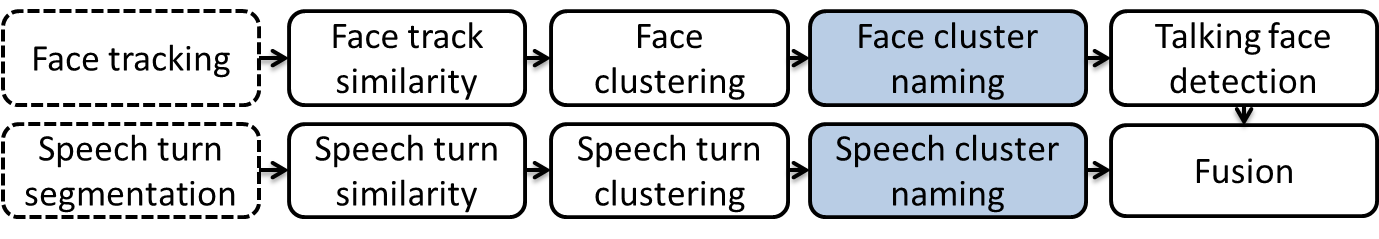
\includegraphics[width=1.\linewidth]{CBN.png}
\vspace*{-5mm}
 \caption{Clustering-based naming process. Light blue boxes are when names are combined with clusters.}
\vspace*{-5mm}
 \label{fig:cbn}
\end{figure}

\subsection{Face clustering}

Given the video shots, face clustering process consists of (i) face detection, detecting faces appearing within each shot, (ii) face tracking, extending detections into continuous tracks within each shot, and (iii) face clustering, grouping all tracks with the same identity into clusters.

\subsubsection{LIMSI system}

Face tracking-by-detection is applied within each shot using a detector based on histogram of oriented gradients~\cite{Dalal2005} and the correlation tracker proposed by \emph{Danelljan et al.}~\cite{Danelljan2014}. 
%
Each face track is then described by its average \emph{FaceNet} embedding and compared with all the others using Euclidean distance~\cite{Schroff2015}. 
%
Finally, average-link hierarchical agglomerative clustering is applied. Source code for this module is available in \emph{pyannote-video}\footnote{\url{http://pyannote.github.io}}.

\subsubsection{EUMSSI system}

A fast version of deformable part-based model (DPM)~\cite{dubout2013deformable} is first applied. Then tracking is performed using the CRF-based multi-target tracking framework~\cite{heili2014tracking}, which relies on the unsupervised learning of time sensitive association costs for different features.
%
The detector is only applied 4 times per second and an explicit false alarm classifier at the track level is learned\cite{Le_ICPR_2016}.
%
Each face track is then described using a combination of keypoint matching distances and total variability modeling (TVM)~\cite{wallace2012total,Khoury:ICMR:2013}.

\subsection{Speaker diarization}

The speaker diarization system (``who speak when?") is based on the LIUM Speaker Diarization system\cite{rouvier2013}, freely distributed\footnote{\url{www-lium.univ-lemans.fr/en/content/liumspkdiarization}}. 
%This system has achieved the best or second best results in the speaker diarization task on REPERE French broadcast evaluation campaigns 2012 and 2013~\cite{galibert2013b}.
%
The diarization system is first composed of an acoustic Bayesian Information Criterion (BIC)-based segmentation followed by a BIC-based hierarchical clustering. Each cluster represents a speaker and is modeled with a full covariance Gaussian. A Viterbi decoding re-segments the signal using GMMs% with 8 diagonal components learned by EM-ML, 
for each cluster. 
%Segmentation, clustering and decoding are performed with 12 MFCC+E, computed with a 10ms frame rate. 
Music and jingle regions are removed using a Viterbi decoding with 8 GMMs (trained on french broadcast news data) for music, jingle, silence, and speech. %(with wide/narrow band variants for the last two, and clean or noised or musical background variants for wideband speech).
%
%In the above steps, features were used unnormalized in order to preserve information on the background environment, which may help differentiating between speakers. 
At this point each cluster contains the voice of only one speaker, but several clusters can be related to a same speaker. The background environment contribution must be removed from each GMM cluster, through feature gaussianization.
%
Finally, the system is completed with clustering method based on the i-vectors paradigm and Integer Linear Programming (ILP)~\cite{rouvier12-2}. 
%This clustering method is fully described in. 
%The ILP clustering along with i-vectors speaker models gives better results than the usual hierarchical agglomerative clustering based on GMMs and cross-likelihood distances~\cite{Barras2006}.

\subsection{Name assignment}

After obtaining homogeneous clusters during which distinct identities speak or appear, one needs to assign each name from NER module to the correct clusters. 
%
%However, associating auditory voices with visual person clusters or names has two major difficulties. 
%The visible person may not be the current speaker and the speaking person can be dubbed by a narrator in a different language.
%
%Because of these problems of AV association, 
We use a direct naming method~\cite{poignant2012fusion} to find the mapping that maximizes the co-occurrences between clusters and names.
%
Names are propagated on the outputs of face clustering and speaker diarization independently. 
%
%The direct naming method is applied to speaker clusters to produce a mapping between names and clusters. All shots which overlap with the clusters are tagged with the corresponding names with equal confident scores. 
%
%The same direct method is applied to face clusters to produce a set of named clusters.
%Unlike speaker naming, for  one shot, 
A name coming from face naming is ranked based on the talking score of the segment within that shot using lip motion and temporal modeling with LSTM~\cite{Le_ACMMM_2016}.

\endinput
